\documentclass{beamer}
\usetheme{Montpellier}
\usepackage{graphicx}
\usepackage{url}
\usepackage{multicol}

\title{Elliptic Curve Cryptography}
\author{Justin Findlay \\ \texttt{jfindlay@gmail.com}}
\date[SLC Python]{2016 January 6}

\begin{document}
\maketitle

\section{Maths}

\subsection{Elliptic Curves}

\begin{frame}
\frametitle{Elliptic Curves}
Weierstrass equation\footnote{\url{https://en.wikipedia.org/wiki/Elliptic_curve}}:
\begin{align*}
  y^2 = x^3 + ax + b
\end{align*}
where
\begin{align*}
  \forall a,b \in \mathbb R && \text{and} && \Delta = -16(4a^3 + 27b^3) \not= 0
\end{align*}
\begin{center}
  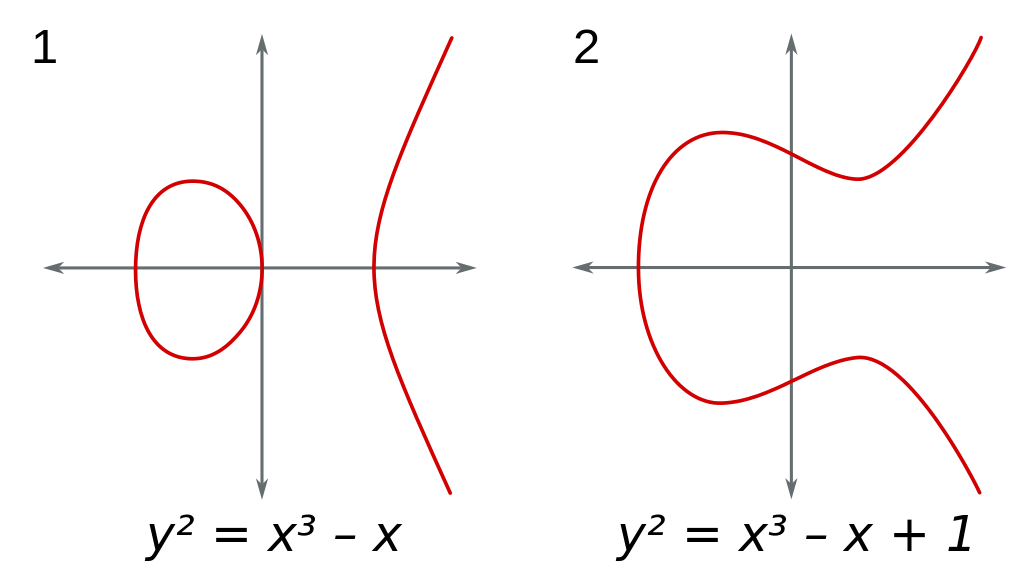
\includegraphics[width=6cm]{elliptic_curves.png}
\end{center}
\end{frame}

\begin{frame}
\frametitle{Utility of Elliptic Curves}
Elliptic curves are related to:
\begin{itemize}
  \item Riemann $\zeta$ function\footnote{And consequently the Riemann hypothesis: \url{https://en.wikipedia.org/wiki/Riemann_hypothesis\#Consequences_of_the_Riemann_hypothesis}}
    \begin{multicols}{2}
      \begin{align*}
        \zeta(s) &= \sum_{n=1}^\infty n^{-1} \\
                 &= \frac{1}{1^s} + \frac{1}{2^s} + \frac{1}{3^s} + \cdots \\
                 &= \frac{1}{\Gamma(s)} \int_0^\infty \frac{x^{s - 1}}{e^x -1}\mathrm d x
      \end{align*}
      \columnbreak
      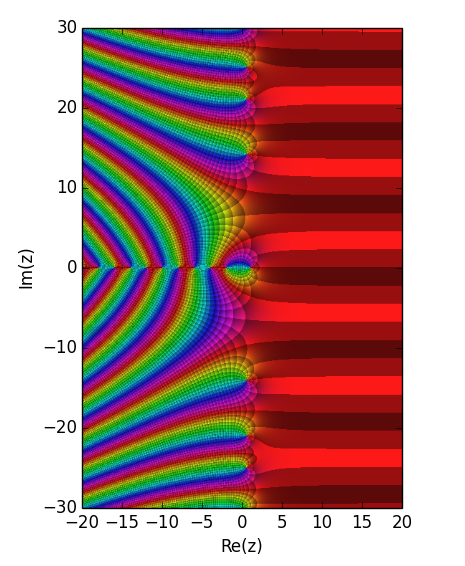
\includegraphics[width=4cm]{Riemann_zeta_function.png}
    \end{multicols}
\end{itemize}
\end{frame}

\begin{frame}
\frametitle{Utility of Elliptic Curves}
Elliptic curves are related to:
\begin{itemize}
  \item Fermat's last theorem
    \begin{align*}
      \forall\ x,y,z \in \mathbb Z, && \exists\ n \in \mathbb Z && \text{such that} && x^n + y^n = z^n
    \end{align*}
  \item Birch and Swinnerton-Dyer conjecture
  \item Langlands Program: Galois groups $\leftrightarrow$ automorphic forms, representation theory, {\it etc}.
  \item Galois Theory
  \item Lie Theory
  \item {\it etc}.
\end{itemize}
\end{frame}

\subsection{Algebra}

\begin{frame}
\frametitle{Groups}
A group is a 2-tuple consisting of a set $G$ and an operation $*$ having a list of properties.

Consider the set of integers and the addition operation, $(\mathbb Z,+)$.  For any $a,b,c \in \mathbb Z$:
\begin{itemize}
  \item Closure: $a + b \in \mathbb Z$
  \item Associativity: $(a + b) + c = a + (b + c)$
  \item Identity: $\exists\ 0 \in \mathbb Z$ such that $a + 0 = a$
  \item Inverse: $\exists\ -a \in \mathbb Z$ such that $a + (-a) = 0$
  \item (Commutativity: $a + b = b + a$, only for abelian groups)
\end{itemize}
\end{frame}

\begin{frame}
\frametitle{Fields}
A field is a 3-tuple consisting of a set $G$ and two operations $\dag,*$ having a list of properties.

Consider the set of rational numbers and the addition and multiplication operations, $(\mathbb Q,+,\times)$.  For any $a,b,c \in \mathbb Q$:
\begin{itemize}
  \item the 2-tuple $(\mathbb Q,+)$ is an abelian group
  \item the 2-tuple $(\mathbb Q \setminus \{0\},\times)$ is an abelian group
  \item Distributivity: $a\times(b + c) = a\times b + a\times c$
\end{itemize}
\end{frame}

\begin{frame}
\frametitle{Vector Spaces}
\begin{multicols}{2}
  A vector space is a 3-tuple of a cartesian product of identical sets and two operations. \\
  \columnbreak
  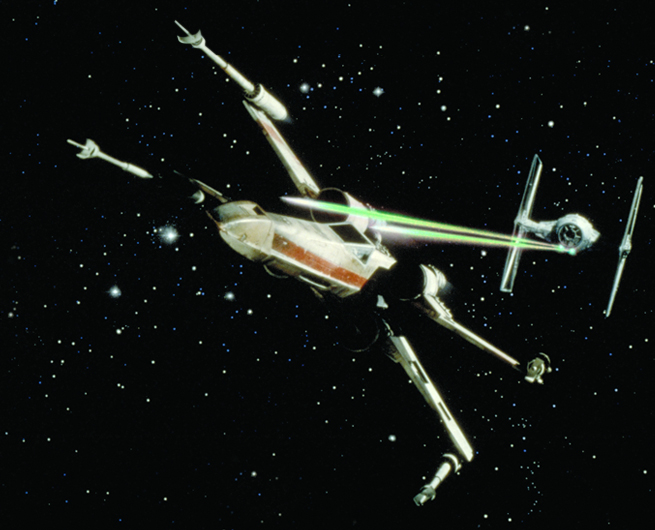
\includegraphics[width=3cm]{X-Wing_TIE.png}
\end{multicols}

Consider the three copies of the set of integers $\mathbb Z\times \mathbb Z\times \mathbb Z = \mathbb Z^3$, vector addition and scalar multiplication, $(\mathbb Z^3,+,\cdot)$.  For any $\pmb u,\pmb v,\pmb w \in \mathbb Z^3$ and $a,b \in \mathbb Z$:
\begin{itemize}
  \item the 2-tuple $(\mathbb Z^3,+)$ is a group
  \item Compatibility: $a\cdot(b\cdot\pmb v) = (ab)\cdot\pmb v$
  \item Scalar Identity: $1\cdot\pmb v = \pmb v$
  \item Field Distributivity: $(a + b)\cdot\pmb v = a\cdot\pmb v + b\cdot\pmb v$
  \item Vector Distributivity: $a\cdot(\pmb v + \pmb u) = a\cdot\pmb v + a\cdot \pmb u$
\end{itemize}
\end{frame}

\begin{frame}
\frametitle{Modular Arithmetic and Finite Fields}
\begin{multicols}{2}
  A finite group or a finite field is a group or a field whose set is finite. \\
  \columnbreak
  
\includegraphics[width=3cm]{modular_arithmetic.png}\footnote{http://pajhome.org.uk/crypt/rsa/maths.html}
\end{multicols}
Examples:
\begin{align*}
  7 + 8 = 15 &\equiv 2 \mod 13 \\
  10\times10 = 20 &\equiv 7 \mod 13
\end{align*}
\end{frame}

\begin{frame}
\frametitle{Projective Plane}
\begin{center}
  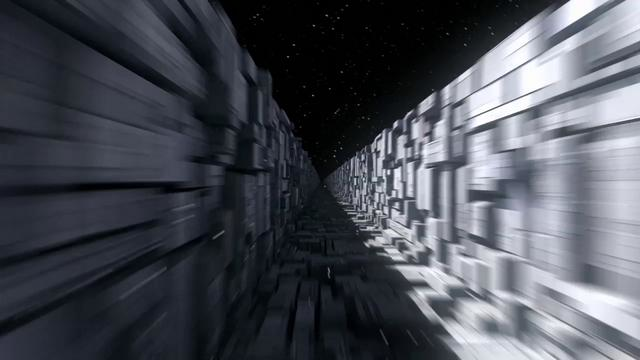
\includegraphics[width=6cm]{Death_Star_trench.png}
\end{center}
The projective plane (the set $\mathbb R^2 + \{P\}$, where $P$ is the point at infinity):
\begin{itemize}
  \item $\forall$ points $a,b \in \mathbb P$, $\exists$ exactly one line $L \subset \mathbb P$ such that $a,b \in L$
  \item $\forall$ lines $K,L \in \mathbb P$, $\exists$ exactly one point $a \in \mathbb P$ such that $a \in L$ and $a \in K$
  \item $\forall a,b,c,d \in \mathbb P$, $\exists$ no line $L \subset \mathbb P$ such that more than two points $\in L$
\end{itemize}
\end{frame}

\begin{frame}
\frametitle{Projective Plane}
\begin{center}
  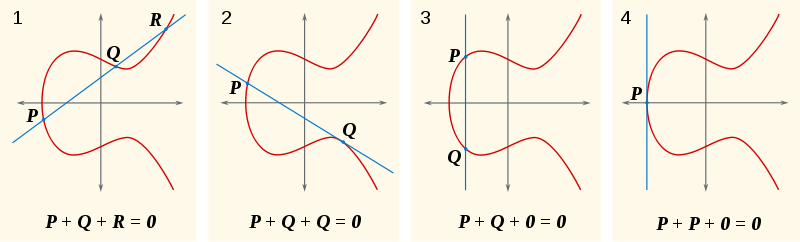
\includegraphics[width=10cm]{elliptic_curve_algebra.png}\footnote{\url{https://en.wikipedia.org/wiki/File:ECClines.svg}}
\end{center}
The projective plane is needed to do algebra over the points on an elliptic curve.  The point at infinity serves as the identity element.
\end{frame}

\begin{frame}
\frametitle{Discrete Logarithm}
\begin{itemize}
  \item The discrete logarithm\footnote{Also see: \url{https://www.khanacademy.org/computing/computer-science/cryptography/modern-crypt/v/discrete-logarithm-problem}}:
    \begin{align*}
      n^k \mod p && k,n,p \in \mathbb Z
    \end{align*}
  \item The discrete logarithm problem:
    \begin{align*}
      n^k \mod p = N \equiv m
    \end{align*}
    Is there a polynomial time algorithm that can find $k$ by knowing $N$?  Whereas finding $N$ by knowing $k$ is easy.
  \item ($n$ is known as a generator of the group $\mathbb Z_p$)
\end{itemize}
\end{frame}

\section{Cryptography}

\begin{frame}
\frametitle{Hashing}
\begin{multicols}{2}
  A hash is a function that maps strings of bytes of arbitrary length into a set of strings of bytes that have relatively short and identical lengths.
  \columnbreak
  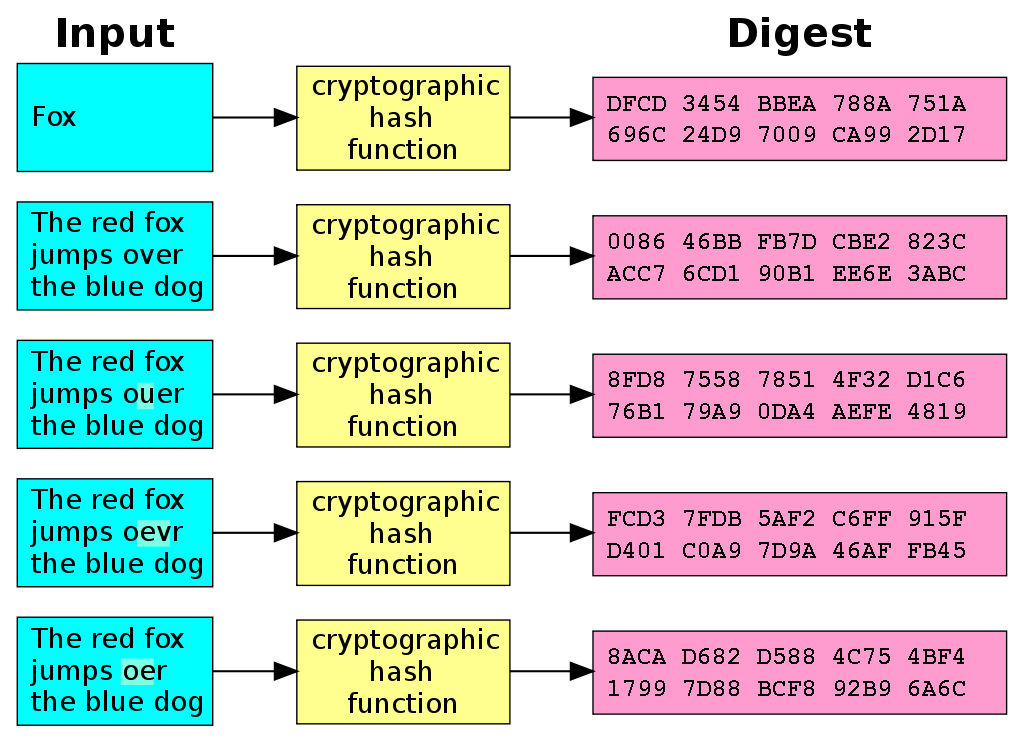
\includegraphics[width=6cm]{hash.png}\footnote{\url{https://commons.wikimedia.org/wiki/File:Cryptographic_Hash_Function.svg}}
\end{multicols}
\end{frame}

\begin{frame}
\frametitle{Symmetric Keys}
\begin{center}
  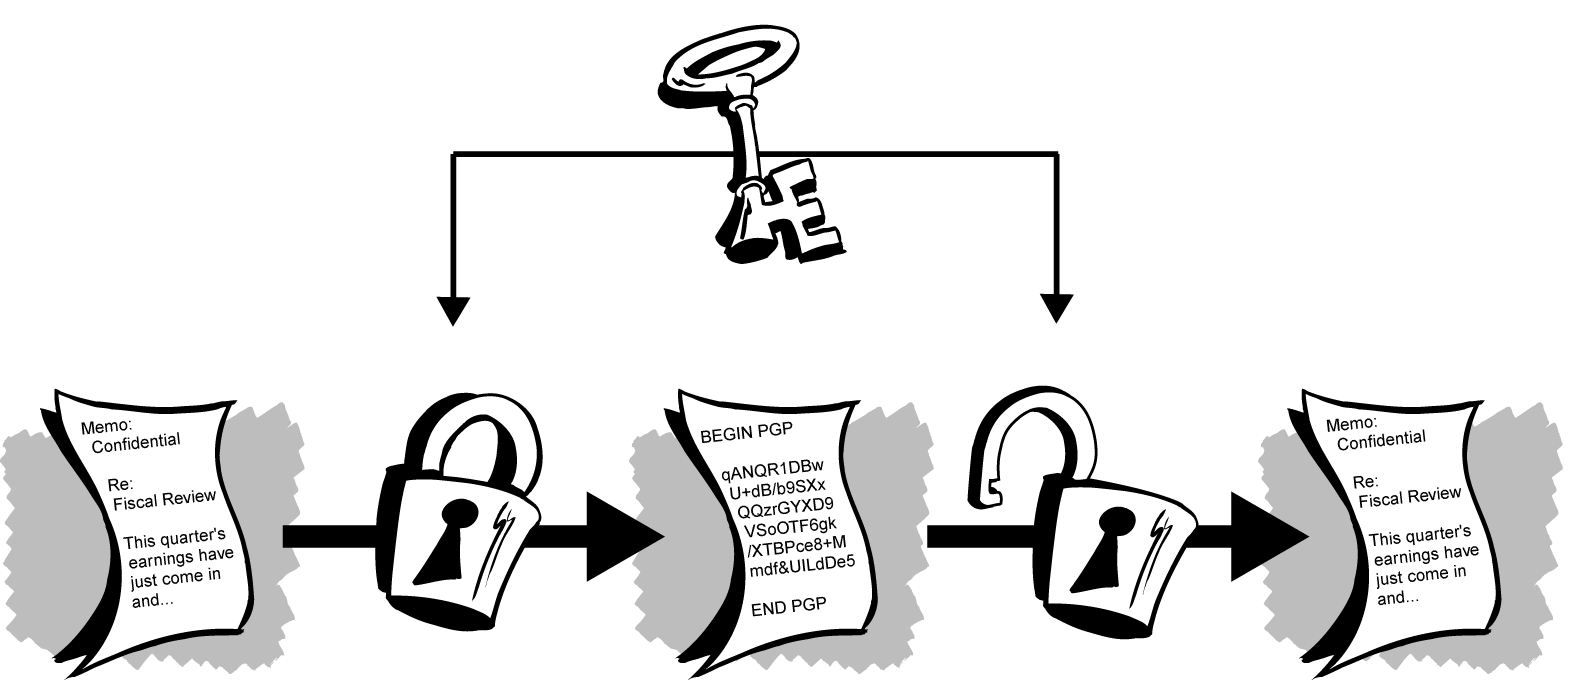
\includegraphics[width=10cm]{symmetric_key.png}\footnote{\url{http://fisher.osu.edu/~muhanna.1/pdf/crypto.pdf}}
\end{center}
\end{frame}

\begin{frame}
\frametitle{Asymmetric Keys}
\begin{center}
  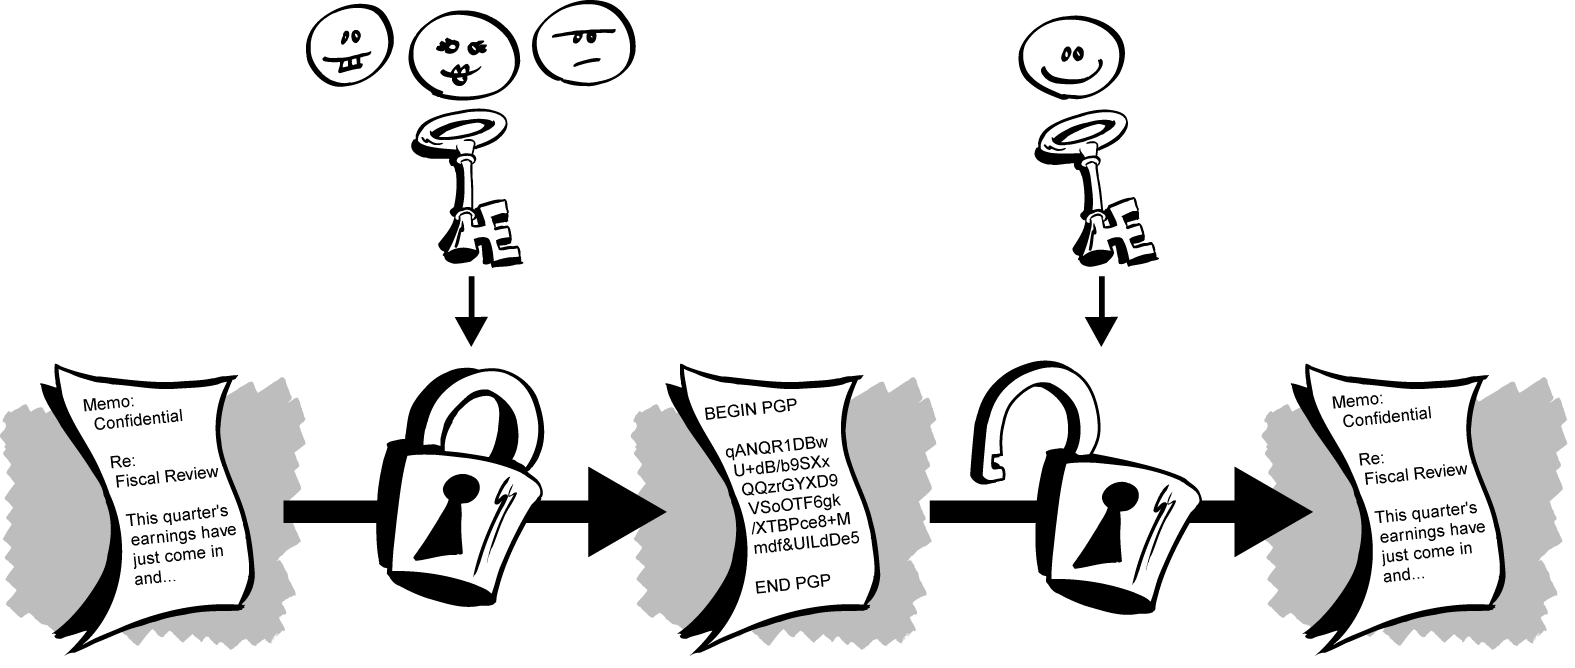
\includegraphics[width=10cm]{asymmetric_keys.png}\footnote{\url{http://fisher.osu.edu/~muhanna.1/pdf/crypto.pdf}}
\end{center}
\end{frame}

\begin{frame}
\frametitle{Signing}
\begin{center}
  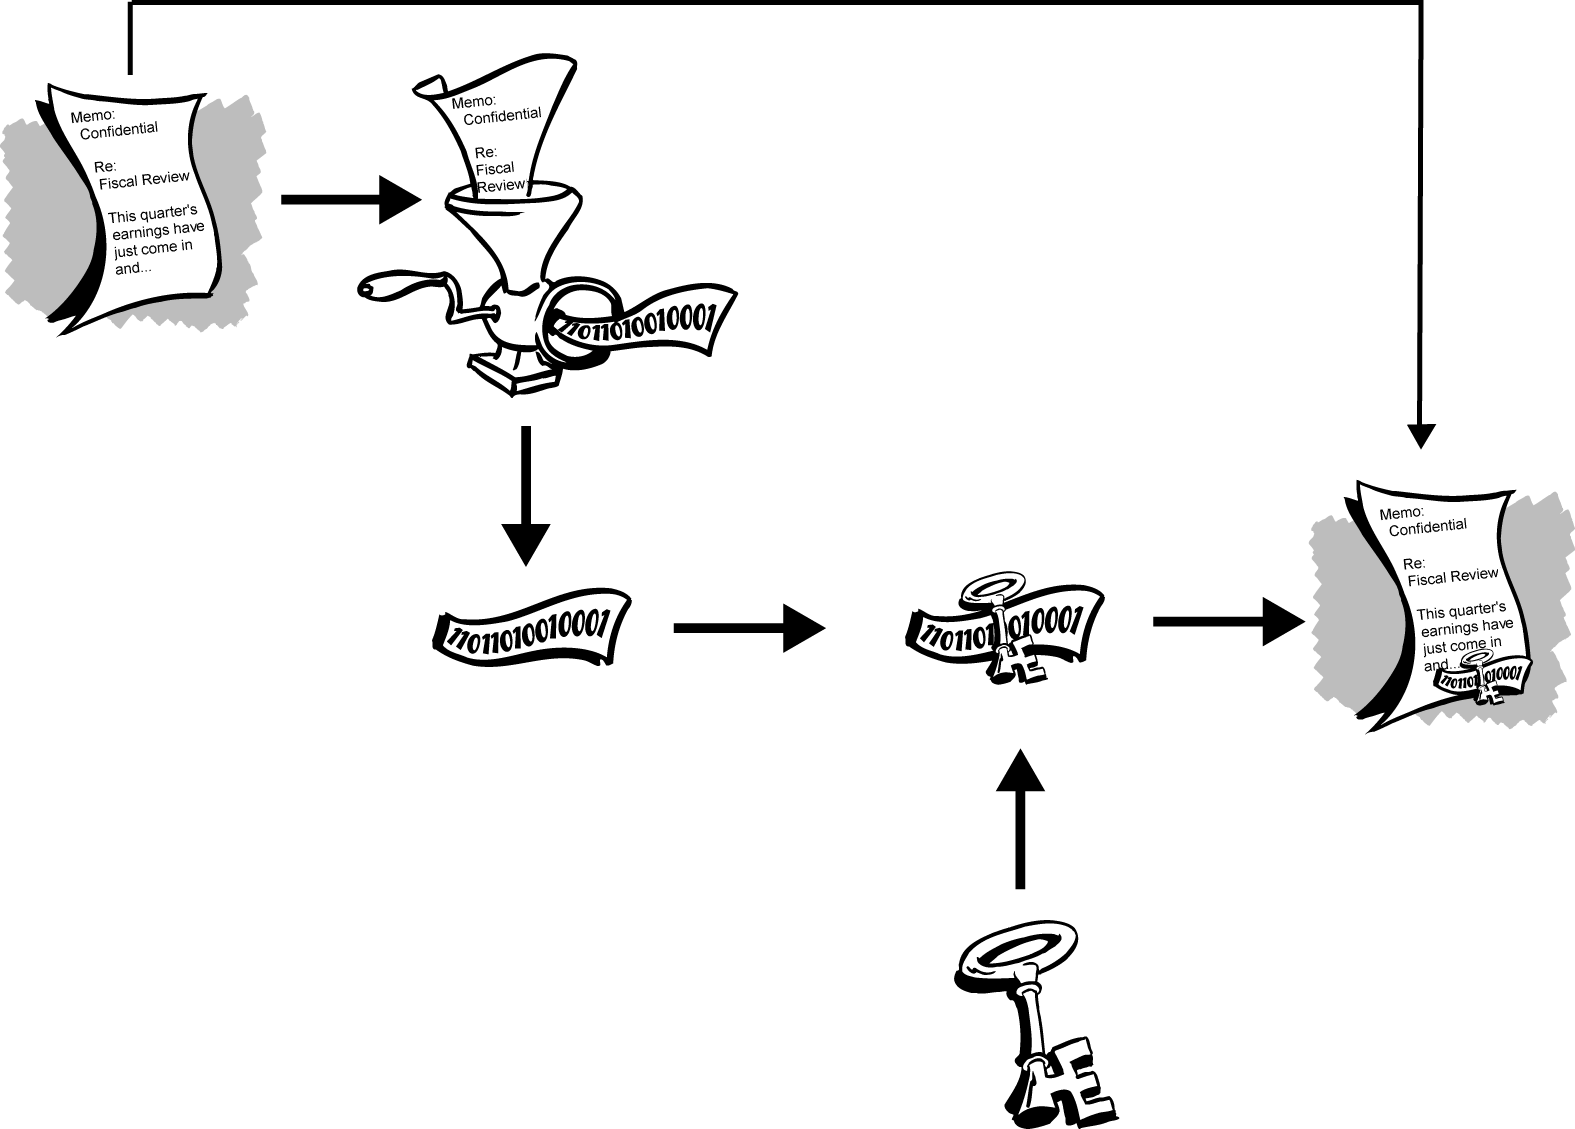
\includegraphics[width=9cm]{signing.png}\footnote{\url{http://fisher.osu.edu/~muhanna.1/pdf/crypto.pdf}}
\end{center}
\end{frame}

\section{Elliptic Curve Crypto Libraries}

\begin{frame}
\frametitle{Libraries}
\begin{itemize}
  \item NaCl
    \begin{itemize}
      \item NaCl: \url{http://nacl.cr.yp.to/}
      \item tweetNaCl: \url{http://tweetnacl.cr.yp.to/}
      \item libsodium: \url{https://github.com/jedisct1/libsodium}
    \end{itemize}
  \item libnacl
    \begin{itemize}
      \item home: \url{https://github.com/saltstack/libnacl}
      \item docs: \url{https://libnacl.readthedocs.org/en/latest/}
    \end{itemize}
  \item PyNaCl
    \begin{itemize}
      \item home: \url{https://github.com/pyca/pynacl}
      \item docs: \url{https://pynacl.readthedocs.org/en/latest/}
    \end{itemize}
  \item pure\_pynacl: \url{https://github.com/jfindlay/pure\_pynacl}
\end{itemize}
\end{frame}

\end{document}
